\documentclass[main.tex]{subfiles}
\begin{document}

\section{Sheet 11}

\subsection{Wave equation}

\subsubsection{General travelling impulse}

We want to show that any twice-differentiable function \(F(z \pm v t) = f(z, t)\) solves the wave equation: 
%
\boxalign{
\begin{align} \label{eq:wave-equation}
\qty(-\partial_{t}^2 + v^2 \partial_{z}^2) f(t, z) = 0
\,. 
\end{align}}

We denote \(\alpha (t,z) = z \pm vt\), so that \(f = F \circ \alpha \) and: 
%
\begin{subequations}
\begin{align}
\pdv[2]{f}{t} = \pdv{}{t }\qty( \dv{F}{\alpha } \pdv{\alpha }{t}) &= \dv{F}{\alpha } \pdv[2]{\alpha }{t} +  \pdv{\alpha }{t} \pdv{}{t} \qty(\dv{F}{\alpha })  \\
&= \dv{F}{\alpha } \pdv[2]{\alpha }{t}
+ \pdv{\alpha }{t}\dv{}{\alpha } \qty(\dv{F}{\alpha } \pdv[]{\alpha }{t}) \marginnote{Commuted the derivatives}\\
&= \dv{F}{\alpha } \pdv[2]{\alpha }{t}
+ \pdv{\alpha }{t} \qty( \dv[2]{F}{\alpha } \pdv[]{\alpha }{t} 
+ \dv{F}{\alpha } \cancelto{}{\pdv{}{t} \dv{\alpha }{\alpha }}) \marginnote{Derivative of a constant}  \\
&= \dv{F}{\alpha } \pdv[2]{\alpha }{t}
+ \dv[2]{F}{\alpha } \qty(\pdv[]{\alpha }{t})^2  \label{eq:faa-di-bruno}\\
&= v^2 \dv[2]{F}{\alpha }
\,,
\end{align}
\end{subequations}
%
where the expression we derived is fully general up to equation \eqref{eq:faa-di-bruno}, while the last passage comes from the fact that \(\pdv*{\alpha }{t} = \pm v\), so its square is \(v^2\) while the second derivative is zero since \(v\) is a constant. By the same reasoning, 
%
\begin{subequations}
\begin{align}
\pdv[2]{f}{z} &= \dv{F}{\alpha } \pdv[2]{\alpha }{z} 
+ \dv[2]{F}{\alpha } \qty(\pdv{\alpha }{z})^2  \\
&= \dv[2]{F}{\alpha }
\,.
\end{align}
\end{subequations}

Therefore, 
%
\begin{align}
\qty(-\partial_{t}^2 + v^2 \partial_{z}^2) f(t, z) 
= (-v^2 + v^2) \dv[2]{F}{\alpha } \equiv 0 
\,.
\end{align}

\subsubsection{Gaussian pulse}

At any fixed time \(t\), the function 
%
\begin{align}
F(\alpha ) = \exp(- \alpha^2) = \exp(- \qty(z - v t)^2)
\,
\end{align}
%
looks like a rescaled Gaussian, centered around \(z = vt\). As \(t\) increases it travels rightward with speed \(v\). A plot of this, with \(v = 6\) and \(t = 0, 1, 2\) is shown in figure \ref{fig:moving-gaussian-pulse}.

\begin{figure}[H]
\centering
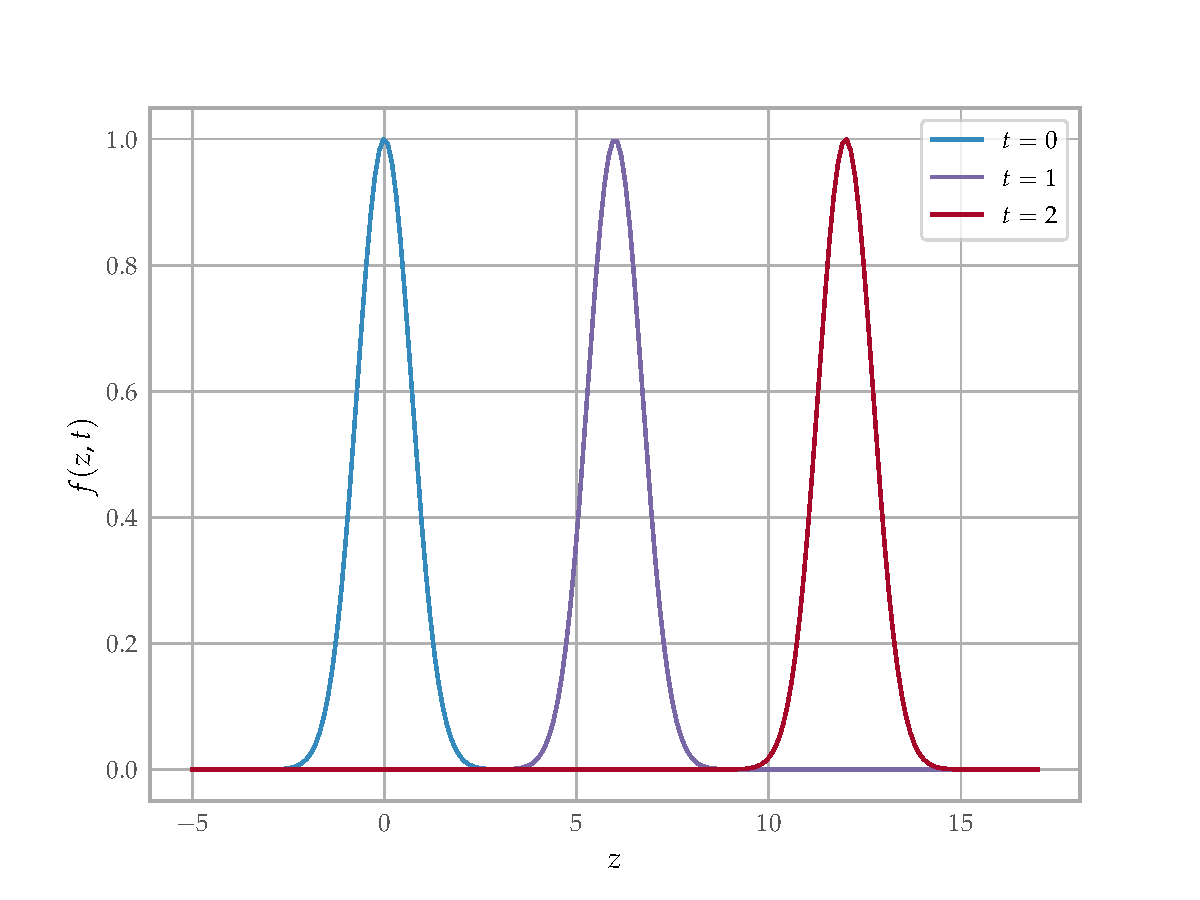
\includegraphics[width=\textwidth]{figures/gauss.pdf}
\caption{Pulse for \(t = 0, 1, 2\).}
\label{fig:moving-gaussian-pulse}
\end{figure}

\subsection{Harmonic wave solution}

We consider the harmonic solution 
%
\begin{align}
f(t,z) 
= A \cos(2 \pi \qty(\frac{z}{\lambda } - \frac{t}{T})) 
= A \cos(\frac{2\pi}{\lambda } \alpha (t,z)) 
\,,
\end{align}
%
where \(\alpha  = z - \lambda t /T\). Writing the harmonic solution this way allows us to see the properties easily: we have \(v  = \lambda / T\) by comparison with the formula from before (\(\alpha = z - vt\)), while the periodicity follows from that of the cosine: we start from the fact that \(\cos(x) = \cos(x \pm 2 \pi )\).

If we map \(z \rightarrow z  + \lambda \) we get \(\alpha \rightarrow \alpha +\lambda \), and 
%
\begin{align}
\cos(\frac{2 \pi }{\lambda } \alpha ) \rightarrow \cos(\frac{2 \pi }{\lambda }\qty(\alpha + \lambda )) = \cos(\frac{2 \pi }{\lambda } \alpha  + 2 \pi ) = \cos(\frac{2 \pi }{\lambda } \alpha )
\,.
\end{align}

Similarly, if we map \(t \rightarrow t + T\) we get \(\alpha \rightarrow \alpha - \lambda T/T = \alpha - \lambda  \), so we can apply the same reasoning. This means that the wave has spatial period \(\lambda \) and temporal period \(T\). 

\subsubsection{Lightspeed waves}

The equation \(\square f = 0\) is analogous to \eqref{eq:wave-equation} for \(v = 1 (= c)\). The difference is the three-dimensionality of the spatial derivatives, however this does not present an issue. 
We still consider solutions in the form \(f (x^{\mu }) = F(\alpha (x^{\mu }) )\), with \(\alpha (x^{\mu }) = k_{\mu } x^{ \mu }\) for a constant covector \(k_{\mu }\). We will have the following derivatives 
%
\begin{align}
\pdv[2]{f}{(x^{\mu })} 
= \dv[2]{F}{\alpha }
\qty( \pdv{\alpha }{(x^{\mu})} )^2
= \dv[2]{F}{\alpha }
\qty(k_{\mu })^2
\,,
\end{align}
%
where the index \(\mu \) can take the conventional values from \(0\) to \(3\). 
So, the equation \(\square f = 0\) reads 
%
\begin{align}
\dv[2]{F}{\alpha } \qty(-\qty(k_{0})^2 + \sum_{i=1 }^{3} \qty(k_{i })^2) = 0
\,,
\end{align}
%
which is always satisfied if we take for  \(k_{\mu }\) a null vector with respect to the Minkowski metric, \(k_{\mu } \eta^{\mu \nu } k_{\nu } = 0 \). 
In order for the wave to be propagating forwards in time we need to set \(k_{0} < 0\), or equivalently \(k^{0}>0\). 

So, the wave equation does indeed have travelling waves as solutions, which propagate with speed 1 (which can be gathered from the factor multiplying the Laplacian). 

\subsection{Gravitational waves}

\subsubsection{Weak-field wave equation}

We consider a perturbed metric \(g_{\mu \nu } = \eta_{\mu \nu } + h_{\mu \nu }\), to first order in \(h_{\mu \nu }\). 

First of all we need to compute the Christoffel symbols: they are given by 
%
\begin{subequations}
\begin{align}
\Gamma^{\mu }_{\nu \rho } 
&= \frac{1}{2} g^{\mu \alpha } \qty(g_{\alpha \nu , \rho } + g_{\alpha \rho , \nu } - g_{\nu \rho , \alpha })  \\
&= \frac{1}{2} g^{\mu \alpha } \qty(h_{\alpha \nu , \rho } + h_{\alpha \rho , \nu } - h_{\nu \rho , \alpha })  \marginnote{\(\eta_{\mu \nu }  \) is constant}  \\
&= \frac{1}{2} \eta^{\mu \alpha } \qty(h_{\alpha \nu , \rho } + h_{\alpha \rho , \nu } - h_{\nu \rho , \alpha })   + \mathcal{O}(h^2) \marginnote{We only consider the first order in \(h\)}
\,.
\end{align}
\end{subequations}

Now, let us look at the Ricci tensor: it is given 
%
\begin{subequations}
\begin{align}
R_{\mu \nu } = R^{\alpha }_{\mu \alpha \nu } 
&= -2 \qty(\Gamma^{\alpha }_{\mu [\alpha , \nu ]}
+ \Gamma^{\beta }_{\mu [\alpha } \Gamma^{\alpha }_{\nu ], \beta })  \\
&= \Gamma^{\alpha }_{\mu \nu , \alpha } - \Gamma^{\alpha }_{\mu \alpha , \nu } + \mathcal{O}(h^2) 
\,,
\end{align}
\end{subequations}
%
\todo[inline]{To be continued\dots}

\end{document}
